\section{PaWS Architecture}

This section presents the general software architecture. At first, the
base and a high-level description of the architecture concept are
introduced. The next subsection describes elements of the PaWS framework
and their relationship. Scenarios of PaWS operations are also included.

\subsection{The \emph{Model-View-Controller} Design Pattern}
\label{mvc}

\begin{figure}[h!]
  \centering
  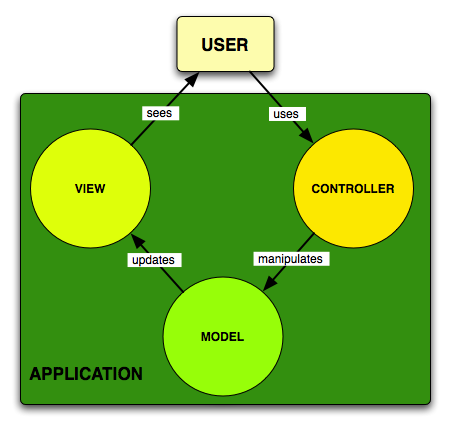
\includegraphics[width=0.5\textwidth]{reportCh2/mvc}
  \caption{MVC concept\cite{mvc_for_php}}
  \label{fig:mvc}
\end{figure}

PaWS is based on the MVC\cite{mvc} design pattern. MVC stands for
\emph{Model-View-Controller} and is an architectural design pattern
for software engineering, especially for creating applications with
graphical user interface.

As can be seen on Figure~\ref{fig:mvc}, MVC divides the application
into three parts:
\begin{itemize}

\item {\bf Model}, which is the representation of the problem or
  application logic,

\item {\bf View}, which describes how to display some parts of the model
  in the user interface,

\item and {\bf Controller}, which is responsible for communicating
  with the user, to update the model and refresh the view.

\end{itemize}

In PaWS framework, the Model layer is not present, because there is no
specific data logic and no database is used. However, PaWS could be
extended by adding, for example, a user authentication or a customization
for users (e.g. memorizing preferences) and, in this case, a database
(and a Model layer) will be necessary.

\subsection{Architecture Overview}

PaWS is a framework which provides its functions remotely. 
\begin{figure}[h!]
  \centering
  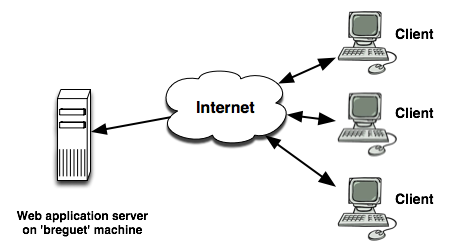
\includegraphics[width=0.5\textwidth]{reportCh2/web_applications}
  \caption{Architecture of access to web applications}
  \label{fig:web_applications}
\end{figure}
This means there is no need to install it on the client machine.  PaWS
can be reached via the Internet as it is shown in the Figure
\ref{fig:web_applications}. Clients need only a web browser - so
called \emph{thin client}. A \emph{Thin client} can be a terminal or a
computer. It needs another machine (its server) to perform its
tasks. Advantages of this approach are 1) no need to install special
tools on client machines, 2) independence from software changes on the
server and 3) low load of the clients machine.

Disadvantages of this solution may be: 1) a reduced functionality
on the client side, 2) the necessity of  an internet connection to
perform the tasks and 3) all of the usual limitations of a network,
latency and bandwidth.

In addition, undre PaWS, PIPS is running, as it is shown in
Figure~\ref{fig:webapp_paws}. What is more, Pyrops, which is described
in section \ref{other_technologies}, enables a remote usage of PIPS and
distribution of the application to balance the load.


\begin{figure}[h!]
  \centering
  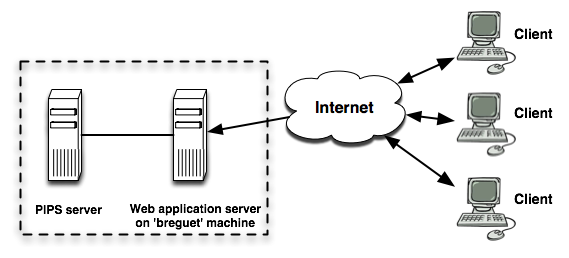
\includegraphics[width=0.5\textwidth]{reportCh2/webapp_paws}
  \caption{Architecture of access to PaWS}
  \label{fig:webapp_paws}
\end{figure}

PaWS architecture is not complicated. It consists of 3 layers,
presented in Figure \ref{fig:paws_architecture}.

\begin{figure}[h!]
  \centering
  
\includegraphics[width=0.7\textwidth]{reportCh2/paws}
  \caption{Architecture of PaWS}
  \label{fig:paws_architecture}
\end{figure}

The top layer is {\bf PaWS web application}. This blue layer consists in:

\begin{itemize}

\item {\bf HTML code} part, which is responsible for the graphical user
  interface. 

\item {\bf Pylons controllers} part, which is responsible for
  interception and interpretation of the user input.

\end{itemize}

The HTML code part is equivalent of the 'View' layer in MVC. HTML
sites are built on the basis of the relevant templates in the
Mako~\cite{} language. Each PaWS mode (like tutorial, basic tools
etc.) has separate templates for creating adequate site. The content
of the WEB pages is specified by a file structure containing the
configuration, e.g. examples or PIPS basic tools. The {\bf
  Ajax}~\cite{} part of this layer is responsible for the dynamic
content of the site and for communicating with the controllers layer,
i.e. for passing variables between those two layers.

The Pylon~\cite{} part can also pass output back to the view layer. Pylons
controllers are a simple and powerful solution. They are special
Python classes, which are very easy to customize. In PaWS, the
controllers layer is also responsible for passing input and getting
back the output of lower layer operations.

The two lower layers of Figure~\ref{fig:paws_architecture} are linked
together very tightly. The yellow middle layer is composed of three
parts. The first of them, {\bf Pylons} is the core of WEB application
and provides all web server functionalities described in
Section~\ref{pylons_descriptions}. The other two parts: PyPS (see:
\ref{pips_and_pyps}) and Tpips (see: \ref{tpips_interface}) are
interfaces for PIPS framework.

The bottom layer is the kernel of the whole system and is composed of
two parts:

\begin{itemize}

\item {\bf Python} (described in \ref{python_description}), which is
  the base for Pylons and PyPS mechanisms.

\item {\bf PIPS core} (described in \ref{pips_and_pyps}), which
  provides all of the transformations and analysis.

\end{itemize}

The middle layer and its interfaces are necessary for the proper
activity of PaWS. Both Tpips and PyPS simplifies usage of PIPS and
encapsulate its main functions and passes. What is more, thanks to
PyPS, it is easy to link Pylons Controllers with PIPS operations. Pyps
can be used to invoke PIPS methods from Python code, directly in the
controller, which goes against a design constraint, or by importing
prepared modules.

\subsection{File Structure}
\label{structure}

The file and directory structure of PaWS consists in two main
parts: the Pylons related part and the PIPS related part.

\begin{figure}[h!]
  \centering
  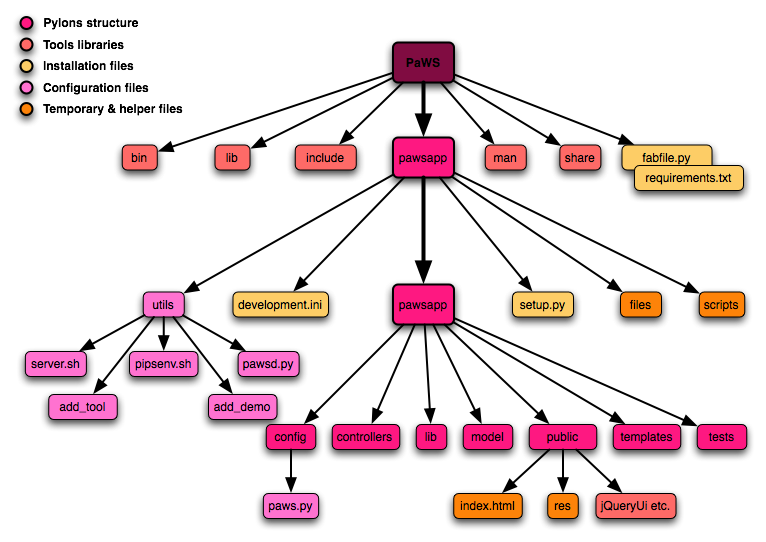
\includegraphics[width=1.0\textwidth]{reportCh2/paws-structure}
  \caption{File structure of PaWS}
  \label{fig:paws_structure}
\end{figure} 

The first one, shown in Figure \ref{fig:paws_structure}, is based on
Pylons directory structure. Files and directories here can
be classified into five types:

\begin{enumerate}

\item {\bf The Pylons} directories which the contain source code
  of PaWS framework. They are described in Section~\ref{architecture_elements}.

\item {\bf The installation files} which are used during the process
  of installation PaWS on a PIPS developper machine. Two of them
  \emph{development.ini} and \emph{setup.py} refer to Pylons directly
  and can be also used as a configuration files. \emph{Fabfile.py} and
  \emph{requirements.txt} are the files of Fabric~\cite{} framework (see
  Section \ref{other_technologies}) designed for quick installation of
  the all dependencies of PaWS framework. More details can be found in
  the section about PaWS installation \ref{installation}.

  \item {\bf The configuration files} - all of the files which can be
    modified by a PIPS developper to get the proper settings for his PaWS
    instance. Scripts used to configurate the application
    content belong to this group too:
    \begin{itemize}
    \item {\bf add\_tool}: a script used to add a new analysis or
      transformation, described in the
      Section~\ref{add_analysis_transformation}.
    \item {\bf add\_demo}: a script used to add a new demonstration,
      described in  Section~\ref{add_demonstration}.
    \item {\bf pipsenv.sh}: a script which adds
      necessary directories to the command path and defines system
      environment variables.
    \item {\bf pawsd.py}: a script which deletes
      old temporary files.
    \item {\bf server.sh}: a script to start application server.
    \end{itemize}

  \item {\bf Temporary and helper files} created by PaWS - directories
    and files which are necessary for PaWS work, but are not the part
    of Pylons architecure. They should not be changed by a PIPS
    developper. Directories \emph{files} and \emph{res} contain
    temporary files created during the PIPS operations. Directory
    \emph{scripts} contains scripts related to adding new
    functionalities of PaWS and the file \emph{index.html} is
    responsible for redirectoring the user to the PaWS introduction
    WEB page.

  \item {\bf Libraries} - directories and files of the tools which
    support work of PaWS, like VirtualEnv, described in
    Section~\ref{virtualenv} or WEB applications technology
    libraries described in Section~\ref{web_application_technologies}.

\end{enumerate}

At the highest level, there are mmostly libraries and binaries related
to the tools used by PaWS, i.e. Virtualenv described in
\ref{virtualenv}.

The second part of PaWS file structure is used for its configuration
by PIPS developper. It is presented in Figure \ref{fig:pips_structure}
and is located in the PIPS \emph{validation} directory. It is mapping
abstract PaWS division into modes, such as tutorial or full control
(described in section \ref{paws_project}) onto the physical
directories structure.

\begin{figure}[h!]
  \centering
  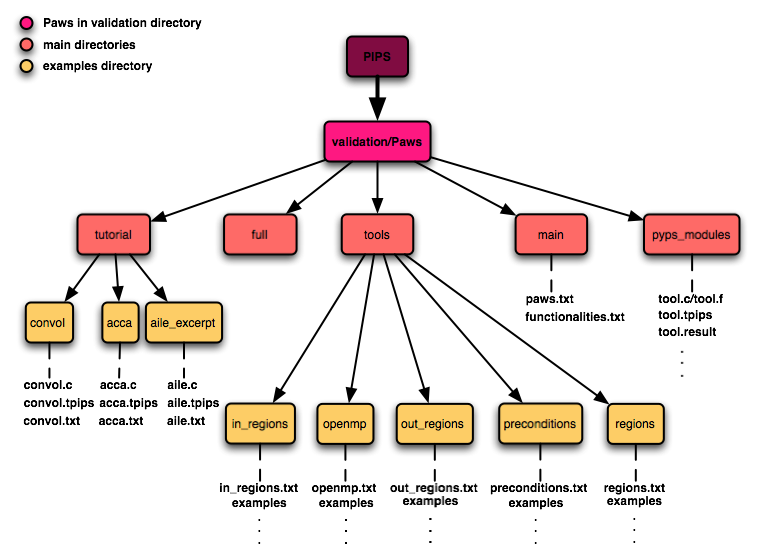
\includegraphics[width=1.0\textwidth]{reportCh2/pips-structure}
  \caption{Structure of PIPS part of PaWS}
  \label{fig:pips_structure}
\end{figure}

\subsection{Architecture elements}
\label{architecture_elements}

This section contains the descriptions of the main types of PaWS
framework elements: controllers, templates, validation directory and
libraries.

\subsubsection{Controllers}

As explained in the previous section, controllers are responsible for
performing actions at the user request. In PaWS several types of
controllers are used.

\begin{enumerate}

\item Controllers responsible for hosting web sites and contains only
  one method ``index''. They are created automatically when adding new
  functionality. Their names correspond to the functionality they
  implement (i.e. ``tools preconditions'' or ``tutorial convol'')

\item Controllers responsible for creating special WEB pages, like the
  ``paas'' controller for the introduction page, or the
  ``descriptions'' controller for extracting information from
  description files.

\item Controllers responsible for the linkage with PyPS or Tpips and
  for performing operations. There are three controllers of this type:
  ``operations'' for basic tools, both at the basic and advanced
  level, ``demo'' for tutorial and ``graph'' for creating dependence
  graps.

\item Controllers for other operations that are not related to PIPS. To
  this group belong the controller ``detector'', which detects the
  language used in source code, and the ``examples'' controller which loads
  supplied examples.

\end{enumerate}

\subsubsection{Templates}

Templates are the files which provide code for WEB pages. They are a
very convenient solution because they let the programmer combine HTML,
Javascript and Python code. What is more, especially when WEB
application consists of many similar pages, templates technology
allows to use the inheritance between templates. That significantly
reduces the amount of redundant code.

PaWS consist of several types of templates:

\begin{itemize}

\item the ``Skeleton'' templates, which provide necessary (and common for
  all of the pages) operations for application to work (like uploading
  files, changing font size or checking if the input source code is
  correct). Those templates (like ``frame'' template) are creating
  structures which are inherited by other, more specific, templates.

\item Templates which are creating frame code dedicated to the
  specific PaWS mode (like tutorial, basic PIPS tools or advanced PIPS
  tools). They are inheriting from more general skeleton templates.

\item Templates which are responsible for creating specific web pages
  dedicated to the special case (one tutorial or PIPS tool). Each of
  them inherits from the appropriate mode template and provides
  characteristic information, such as the name of the PIPS tool or the
  name of a tutorial file.

\item The ``Paas'' template which is responsible for the introduction page,
  and for extracting information about available tools from the
  description files.

\end{itemize}

\subsubsection{Other Modules}
\label{other_modules}

PaWS consists also of some other modules:

\begin{itemize}

\item {\bf \emph{validation}} is the directory of the PIPS project where
  all the supplied examples are placed. All of them
  undergo each day a validation. PaWS validation directory is placed in PIPS
  repository in \emph{validation/Paws} and consists of several
  sub-directories:

  \begin{itemize}

    \item {\bf \emph{pyps\_modules}} described below;

    \item {\bf \emph{tutorial}} which contains all of the demonstration examples;
    \item {\bf \emph{tools}} which contains subdirectories with
      examples dedicated to concrete tool (like \emph{preconditions}
      or \emph{openmp}). Those directories are named after the mode they
      refer to;

  \end{itemize}

\item {\bf PyPS modules} are the part of \emph{validation} directory
  (named \emph{pyps\_modules}). Each module contains PyPS code
  necessary to perform some analysis or transformation. As all of the
  cases kept in \emph{validation} directory because those modules also
  should undergo validation each day.

  \item {\bf \emph{public}} is the Pylons directory where all of the
    helpers but not directly connected to the Pylons or PIPS tools and
    features are placed. In example, all of the Javascript libraries,
    images used by PaWS or description files are stored here.

  \item {\bf \emph{lib}} is the Pylons directory for all of the helper
    Python libraries and modules used by PaWS (like the base Pylons
    controller, the helper for managing files or detection of programming
    languages).

  \item {\bf \emph{tests}} is the Pylons directory for functional
    tests of controllers.

\end{itemize}

\subsection{Flows and scenarios}

This section shows how different elements of PaWS architecture are
linked together. The basic flows for each mode are presented and
described here. Each mode has several cases, different tools or
different demo examples, but in each case the scenario of operations
performed remains the same.

\begin{figure}[h!]
  \centering
  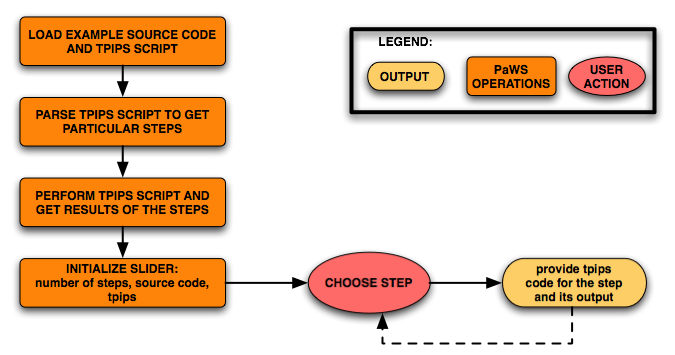
\includegraphics[width=0.7\textwidth]{reportCh2/tutorial_flow}
  \caption{Tutorial flow mode}
  \label{fig:tutorial_flow}
\end{figure}

\begin{itemize}

\item {\bf Demo mode}: there are three scenarios available:
  \emph{aile\_excerpt}, \emph{convol} and \emph{acca-2011}. Input and
  all of the possible operations and their sequence are provided by
  the application - user only controls the step. The basic flow is
  presented on the Picture \ref{fig:tutorial_flow}.
  
  \begin{figure}[h!]
  \centering
  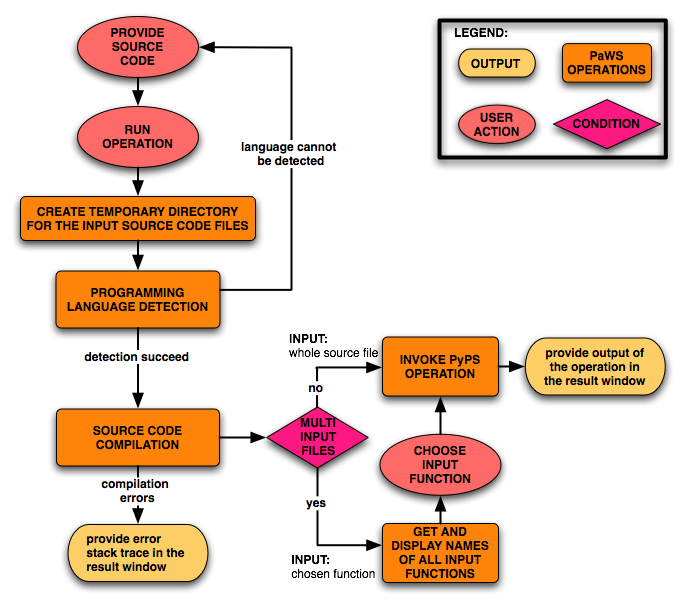
\includegraphics[width=0.7\textwidth]{reportCh2/basic_tool_flow}
  \caption{Basic tool flow mode}
  \label{fig:basic_tool_flow}
\end{figure}

\begin{figure}[h!]
  \centering
  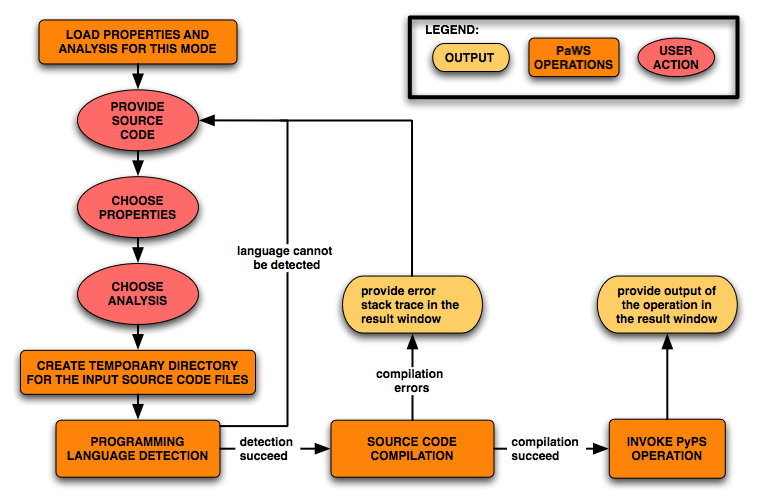
\includegraphics[width=0.7\textwidth]{reportCh2/advanced_tool_flow}
  \caption{Advanced tool flow}
  \label{fig:advanced_tool_flow}
\end{figure}
  
\item {\bf Basic tools - basic level}: five tools are currently
  configured: \emph{preconditions}, \emph{IN regions}, \emph{OUT
    regions}, \emph{regions} and \emph{OpenMP}. This PaWS mode allows
  user to either choose one of supplied examples, different for each
  type of tools, or to provide input source code by him/herself (by
  uploading file or by directly typing or cut-and-pasting in
  application window). The basic flow of this mode is shown in the
  Picture~\ref{fig:basic_tool_flow}.

\item {\bf Basic tools - advanced level}: there are two tools
  available: \emph{preconditions} and \emph{regions}. This mode is
  similar to the basic level - source code can be provided in the same
  way here. The basic scenario is displayed in Picture~\ref{fig:advanced_tool_flow}.
  
  \item {\bf Full control}: not specified and not implemented yet.

\end{itemize}
